\documentclass[12pt]{article}
\usepackage{amssymb}
\usepackage[UTF8]{ctex}
\usepackage{geometry}
\usepackage{units}
\usepackage{pifont}
\geometry{
	a4paper,
	total={150mm,237mm},
	left=30mm,
	top=27mm,
	}
\usepackage{amsmath}
\usepackage{enumerate}
\usepackage{lipsum}
\usepackage{graphicx}
\usepackage{hyperref}
\usepackage{indentfirst}
\usepackage[graphicx]{realboxes}
\usepackage{booktabs}
\usepackage{cases}
\usepackage{subfig}  
\usepackage{float}

\setlength{\parindent}{2em}
\title{HW2}
\author{姓名:陈锐林,学号:21307130148}
\date{\today}

\begin{document}
\maketitle
\begin{LARGE}
    \noindent Chapter4\\
\end{LARGE}
\begin{large}
    Question1:\\
\end{large}
\hspace*{2em}执行代码 "python3 process-run.py -l 5:100,5:100" 后,CPU利用率应该是100\%,因为在该程序中的"<x:y>",x是指令数,y是使用到CPU的占比。而这里两个进程占比都是100\%。使用-c查看也如此:
\begin{figure}[h]
    \centering
    \includegraphics*[height=5cm,width=13cm]{HW2-1.jpg}
\end{figure}\\
\begin{large}
    Question2:\\
\end{large}
\hspace*{2em}首先在该实验中假定I/O处理需要5时间,执行代码 "python3 process-run.py -l 4:100,1:0" 后,前4条指令用时4,后一条从io开始、处理、结束,共需时间7。所以总时间为11。-c查看后符合:
\begin{figure}[h]
    \centering
    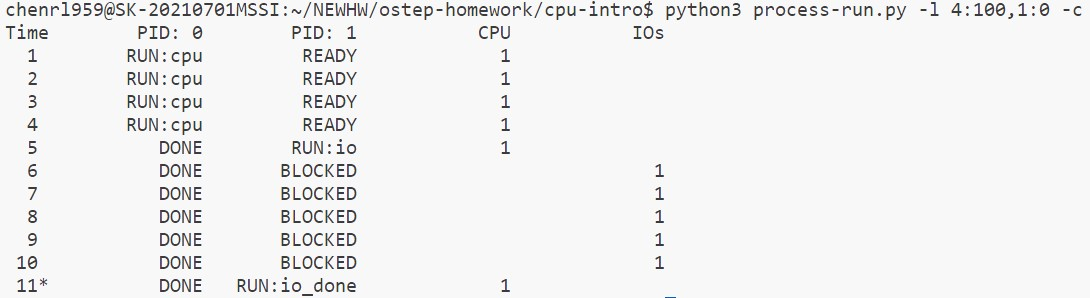
\includegraphics[height=5cm,width=13cm]{HW2-2.jpg}
\end{figure}
\newpage
\begin{large}
    \noindent Question3\\
\end{large}
\hspace*{2em}交换了执行顺序之后,应该出现CPU在两个进程中切换,因为IO被堵塞期间是可以拿来处理第二个进程的指令的。这时候所用时间为1+5(后一进程执行4)+1=7。-c查看后符合:
\begin{figure}[h]
    \centering
    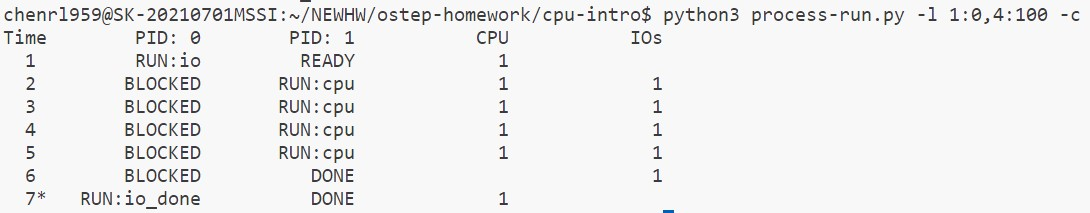
\includegraphics[height=4cm,width=13cm]{HW2-3.jpg}
\end{figure}\\
\begin{large}
    \noindent Question4\\
\end{large}
\hspace*{2em}如果更改标签"SWITCH\_ON\_END",即CPU不会在一个进程完成前切换,所以仍然执行上面的指令,时间还会是Question2中的11。-c查看后符合:
\begin{figure}[h]
    \centering
    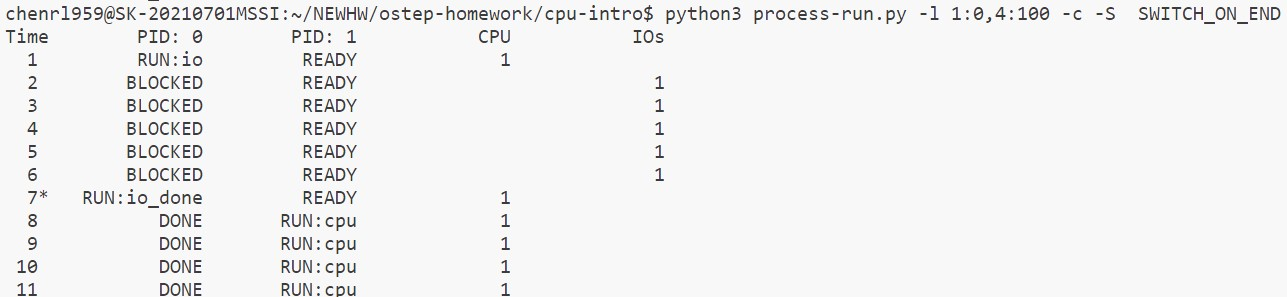
\includegraphics[height=5cm,width=13cm]{HW2-4.jpg}
\end{figure}\\
\begin{large}
    \noindent Question5\\
\end{large}
\hspace*{2em}如果更改标签"SWITCH\_ON\_IO",即CPU会进行切换,所以会回到Question3中的时间7。-c查看后符合:
\begin{figure}[h]
    \centering
    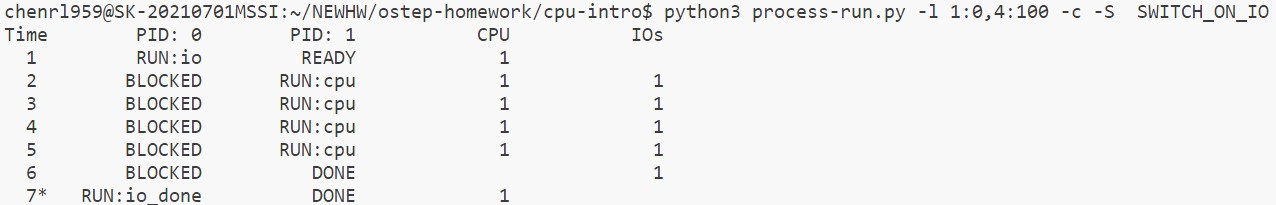
\includegraphics[height=4cm,width=13cm]{HW2-5.jpg}
\end{figure}\\
\newpage
\begin{large}
    \noindent Question6\\
\end{large}
\hspace*{2em}这个问题中有4个进程,通过改标签我们让I/O完成时发出的进程不会马上执行,这会导致:I/O准备好了,但是CPU仍然在执行其他进程,最后无法很好地利用I/O堵塞的时间,导致额外的时间开销。-c查看后符合:首个进程的I/O堵塞多在后面,最后CPU和IO利用率惨淡。
\begin{figure}[h]
    \centering
    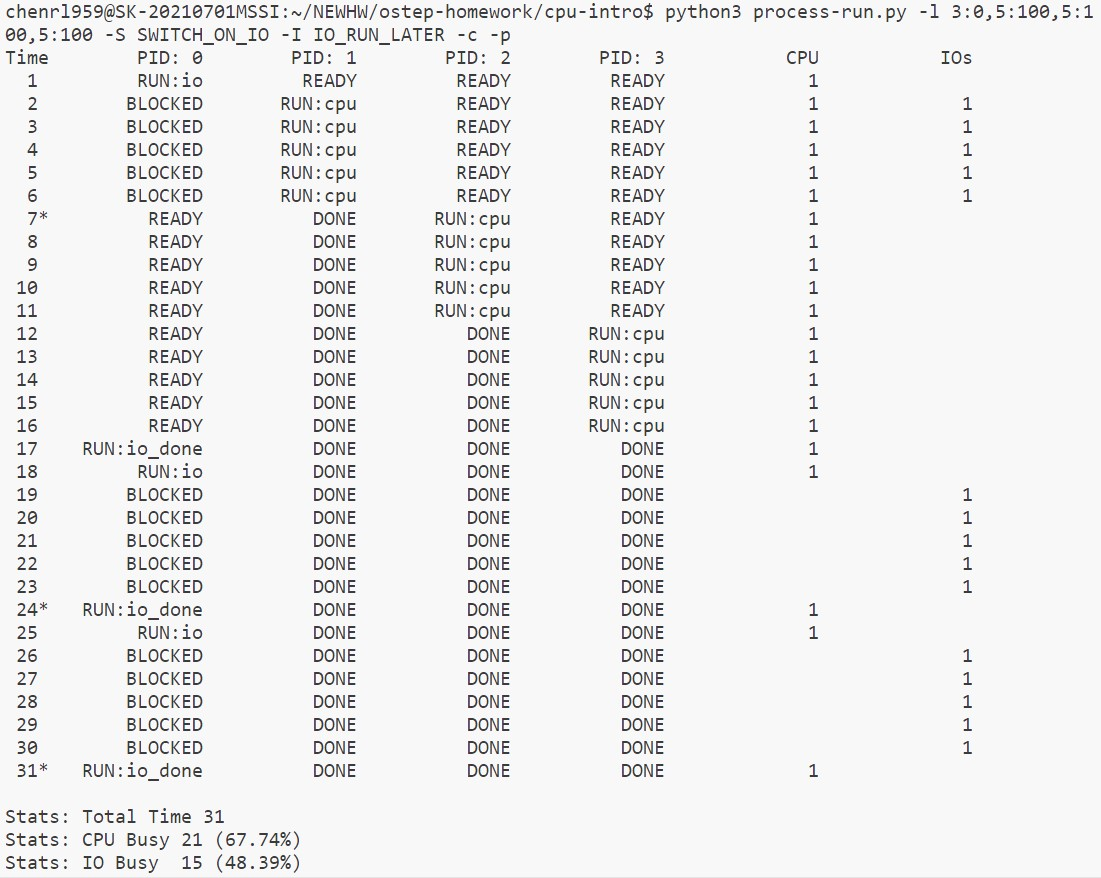
\includegraphics[height=13cm,width=13cm]{HW2-6.jpg}
\end{figure}\\
\begin{large}
    \noindent Question7\\
\end{large}
\hspace*{2em}和Question6相比,这里很明显会使得总耗时最短。因为这样我们能保证利用到I/O的首个进程更快地开始下一条指令,保证先进入I/O的堵塞再切换进程,达到更短的时间。-c后符合:此时CPU利用率最高,CPU在不同的进程间游龙,自由切换。
\newpage
\begin{figure}[h]
    \centering
    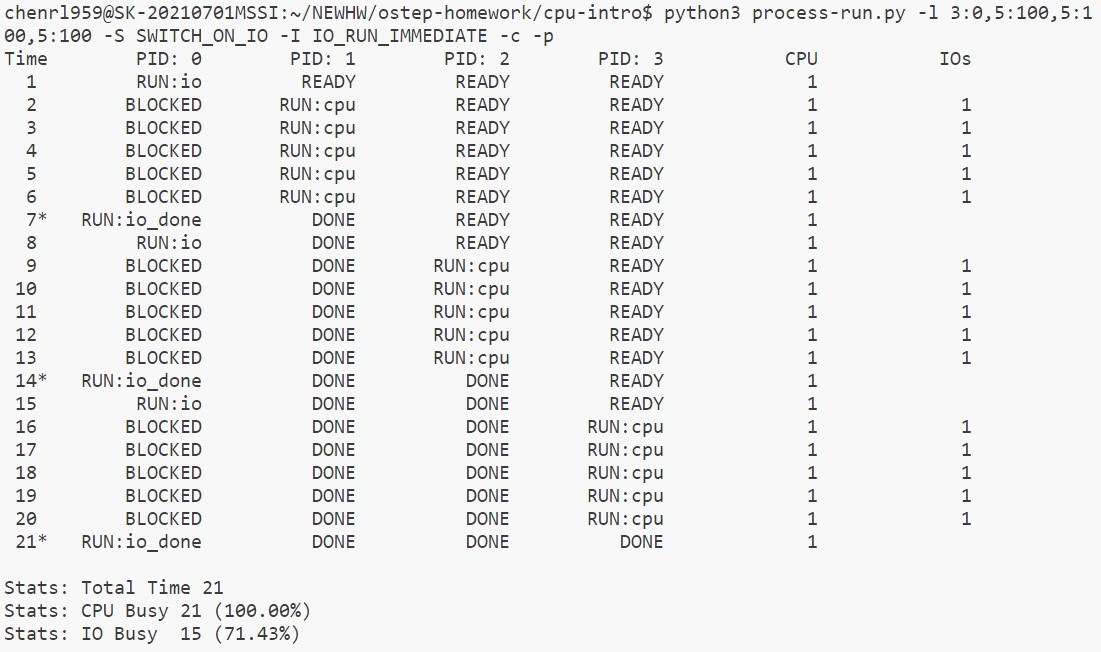
\includegraphics[height=9cm,width=13cm]{HW2-7.jpg}
\end{figure}
\begin{large}
    \noindent Question8\\
\end{large}
\hspace*{2em}对于题目给出的这几组随机生成进程,我都进行了尝试,最后结果如下,该结果表明:使用IO\_RUN\_IMMEDIATE往往会表现得比IO\_RUN\_LATER更佳,使用SWITCH\_ON\_IO会比SWITCH\_ON\_END更佳。效果更佳即有更短的执行时间和更高的CPU利用率。\\
\vspace*{2cm}
\begin{tabular}{p{2cm}p{3cm}p{3.5cm}p{2cm}p{2cm}}  % 其中,tabular是表格内容的环境;c表示centering,即文本格式居中;c的个数代表列的个数
    \toprule[2pt]
    seed & IO\_RUN\_() & SWITCH\_ON\_() & Total Time & CPU busy \\ %中间用 & 隔开, 换行用\\
    \midrule[2pt]
    1    & LATER       & IO             & 15         & 53.3\%   \\
    1    & LATER       & END            & 18         & 44.4\%   \\
    1    & IMMEDIATE   & END            & 18         & 44.4\%   \\
    1    & IMMEDIATE   & IO             & 15         & 53.3\%   \\
    2    & LATER       & IO             & 16         & 62.5\%   \\
    2    & LATER       & END            & 30         & 33.3\%   \\
    2    & IMMEDIATE   & END            & 30         & 33.3\%   \\
    2    & IMMEDIATE   & IO             & 16         & 62.5\%   \\
    3    & LATER       & IO             & 18         & 50.0\%   \\
    3    & LATER       & END            & 24         & 37.5\%   \\
    3    & IMMEDIATE   & END            & 24         & 37.5\%   \\
    3    & IMMEDIATE   & IO             & 17         & 52.9\%   \\
    \bottomrule[2pt]
\end{tabular}
\newpage
\begin{LARGE}
    \noindent Chapter5\\
\end{LARGE}
\begin{Large}
    \noindent 说明\\
\end{Large}
\hspace*{2em}这章的作业都要求fork后在父进程/子进程中执行操作,为了避免冗余,不贴完整代码,只会在每题里说明父进程/子进程分别做了什么操作。\\

\begin{large}
    \noindent Question1\\
\end{large}
\hspace*{2em}这题是最基本的,我设一变量t,初始化为100,在父进程中$t=t/2$,在子进程中$t=t*2$,然后输出结果。我们会发现两个进程对t的改变是互不干扰的,在两个进程刚开始时,t都等于初始值100。运行结果如下:
\begin{figure}[h]
    \centering
    \includegraphics*[height=3cm,width=7cm]{HW2-8.jpg}
\end{figure}\\
\begin{large}
    \noindent Question2\\
\end{large}
\hspace*{2em}这题先打开一个文件描述符,"fd = open("./q2.txt",O\_CREAT|O\_RDWR|O\_\\TRUNC,S\_IRWXU)"。在子进程和父进程中,都调用write,写入不同的信息。我们会发现两个进程都是可以调用fd的,并发写入时,输入都会被保留。运行结果如下:
\begin{figure}[h]
    \centering
    \includegraphics*[height=1.5cm,width=6cm]{HW2-9.jpg}
\end{figure}
\begin{figure}[h]
    \centering
    \includegraphics*[height=2cm,width=6cm]{HW2-10.jpg}
    \caption*{q2.txt中}
\end{figure}\\
\begin{large}
    \noindent Question3\\
\end{large}
\hspace*{2em}题目要求不使用wait确保子进程先输出,最简单的操作就是在父进程输出前调用系统函数sleep(1),1s足够子进程先输出。输出效果即子进程很快打印信息,而父进程等待1s后才打印。
\newpage
\begin{large}
    \noindent Question4\\
\end{large}
\hspace*{2em}经过试验,子进程中能尝试题目中exec()的6个变体,调用形式如下。其中,针对不同函数要准备不同的参数,以e结尾意味着可以改变运行环境,此处不改变就用main后的argv代替;其他的参数类似,args表示"ls","-a"。最后的输出结果类似,如下:
\begin{figure}[h]
    \centering
    \includegraphics*[height=4cm,width=7cm]{HW2-12.jpg}
\end{figure}
\begin{figure}[h]
    \centering
    \includegraphics*[height=2.5cm,width=15cm]{HW2-11.jpg}
\end{figure}\\
\begin{large}
    \noindent Question5\\
\end{large}
\hspace*{2em}根据课上学到的知识,wait会返回等待的pid。这里运行两次,第一次是父进程wait(),检查返回值发现和fork的pid一样;第二次子进程wait(),会发现返回-1。结果如下:
\begin{figure*}[!h]
    \centering
    \subfloat[父wait]{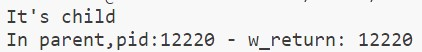
\includegraphics[width=6cm,height=1.5cm]{HW2-13.jpg} \label{X}}
    \hfill
    \subfloat[子wait]{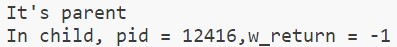
\includegraphics[width=6cm,height=1.5cm]{HW2-14.jpg} \label{Y}}
\end{figure*}\\
\begin{large}
    \noindent Question6\\
\end{large}
\hspace*{2em}换成waitpid后,waitpid参数更多,能执行更多操作,如非阻塞的wait,还可以根据pid等待指定进程。waitpid调用如下:"w = waitpid(pid,NULL,0)"。执行结果和Question5区别不大,子进程waitpid返回-1,父进程返回子进程pid。
\newpage
\begin{large}
    \noindent Question7\\
\end{large}
\hspace*{2em}关闭标准输出后,子进程将不能打印信息,而父进程不受影响。关闭标准输出:"close(STDOUT\_FILENO)",之后终端上只会打印 "It's parent"。
\begin{figure}[h]
    \centering
    \includegraphics*[height=6cm,width=7cm]{HW2-16.jpg}
\end{figure}\\
\begin{large}
    \noindent Question8\\
\end{large}
\hspace*{2em}这题类似之前的Lab1,但较为简单,最主要的工作在子进程中再一次fork,然后进行write和read操作。只需要注意要关闭不用的管道(write时的fd[0],read时的fd[1])。
\begin{figure}[h]
    \centering
    \includegraphics*[height=9cm,width=14cm]{HW2-17.jpg}
\end{figure}
\end{document}